\documentclass{amsart}
\usepackage[dvipsnames,table,xcdraw]{xcolor}
\usepackage{amsmath,amsthm,mathtools}

\usepackage{tikz, pgf}
\usetikzlibrary{matrix, calc, backgrounds, arrows.meta}
\usepackage{tikz-3dplot}
\usepackage{tkz-euclide}
\usepackage{pgfplots}
\usepackage{pgfplotstable}
\pgfplotsset{compat=1.8}
\pgfrealjobname{minimal}

\begin{document}
\beginpgfgraphicnamed{tikz_computers}
    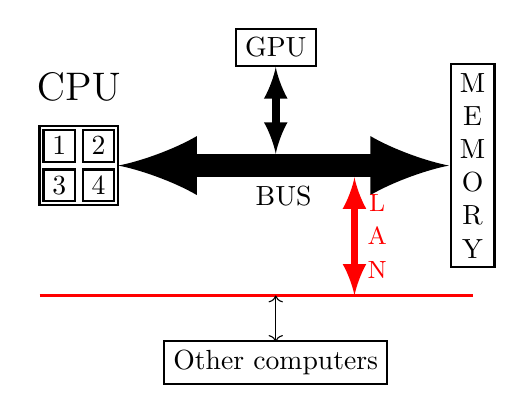
\begin{tikzpicture}
        % define CPU
        \coordinate (CPU_BLC) at (-0.5,-0.5);
        
        % draw CPU
        % \draw[thick] (CPU_BLC) rectangle node[black,above] {CPU} ++(1,1) ;
        \draw[thick] (CPU_BLC) rectangle ++(1,1);
        \draw[thick] (CPU_BLC) ++(0.05,0.05) rectangle 
            ([shift={(0.45,0.45)}]CPU_BLC);
        \draw[thick] (CPU_BLC) ++(0.05,0.55) rectangle 
            ([shift={(0.45,0.95)}]CPU_BLC);
        \draw[thick] (CPU_BLC) ++(0.55,0.05) rectangle 
            ([shift={(0.95,0.45)}]CPU_BLC);
        \draw[thick] (CPU_BLC) ++(0.55,0.55) rectangle 
            ([shift={(0.95,0.95)}]CPU_BLC);

        \node at ([shift={(0.25,0.75)}]CPU_BLC) {1};
        \node at ([shift={(0.75,0.75)}]CPU_BLC) {2};
        \node at ([shift={(0.25,0.25)}]CPU_BLC) {3};
        \node at ([shift={(0.75,0.25)}]CPU_BLC) {4};

        \node at ([shift={(0.5,1.5)}]CPU_BLC) {\Large{CPU}};

        \coordinate (CPU_mem_line_begin) at ([shift={(1,0.5)}]CPU_BLC);

        % define Memory
        \coordinate (Memory) at (5,0);
        \node at (Memory) [draw,thick, align=center] {M\\E\\M\\O\\R\\Y};

        % Define bus
        \draw[latex-latex, line width=3mm] (CPU_mem_line_begin) -- ([xshift=-3mm]Memory) node[midway, below] {BUS};

        % GPU
        \coordinate (GPU) at (2.5,1.5);
        \node at (GPU) [draw, thick] {GPU};

        \draw[latex-latex, line width=1mm] ([yshift=-2.5mm]GPU)-- ++(0,-1.1);

        % LAN
        \coordinate (LAN) at (3.5,0);
        \draw[red, latex-latex, line width=1mm] ([yshift=-1.5mm]LAN) -- ++(0,-1.5) node[midway, right, align=center] {\small{L}\\\small{A}\\\small{N}};

        \draw[red, thick] ([shift={(0,-1.15)}]CPU_BLC) -- ([shift={(5.5,-1.15)}]CPU_BLC);

        \coordinate (Other_Comp) at (2.5, -2.5);
        \node at (Other_Comp) [draw, thick] {Other computers};

        \draw[<->] ([yshift=2.6mm]Other_Comp)--([yshift=8.5mm]Other_Comp);
    \end{tikzpicture}
\endpgfgraphicnamed
\end{document}